\chapter{Industrial Context and Research Framework}
\minitoc

In this first chapter, we present the industrial context in which this research project is inscribed. Primarily, we will review the Industry 4.0 paradigm as well as the benefits it can bring to the manufacturing industry through the application of Machine Learning based data-driven methods. Subsequently, we will describe our industrial research framework, the Extrusion Blow-Molding, and we will rely on an initial bibliographic research work in order to be able to position ourselves scientifically and to formalise our research work. Finally, the goal of this research work is presented: the quality improvement of the fuel tank produced through the Extrusion Blow-Molding process.  

\section{Industry 4.0: a promise for improved manufacturing}

Automotive industry is nowadays driven by global competition and the need for fast adaptation of production to the ever-changing market requests. The fourth revolution in industry, Industry 4.0, holds the promise of increased flexibility in manufacturing, along with mass customisation, better quality, and improved productivity \citep{zhong2017intelligent}. As already occurred for the past three revolutions, technical innovations and a new way of perceiving the world, are radically changing the industry. The first industrial revolution at the end of the 18th century introduced steam-powered machines. The second one used electricity to improve productivity and to create mass production. Electronics and information technology, with the introduction of Programmable Logic Controllers (PLC) began the industrial automation and the third industrial revolution. The context of billions of people connected by mobile devices, with unprecedented processing power, storage capacity, and access to knowledge is promoting the emergence of new technologies. Artificial intelligence, robotics, autonomous vehicles, 3-D printing, nanotechnology, biotechnology, materials science, energy storage, and quantum computing are changing the world and today we are on the cusp of the fourth industrial revolution \citep{schwab20164th}.  

The term Industry 4.0 refers to the connection among production departments, tools, machines, “individual things” in general made possible by Internet and CPS (cyber physical systems) \citep{schlapfer2015industry} .
With the digital revolution, the boundaries between the physical and digital worlds are disappearing to create an interconnected factory with strong interactions between employees, machines and products. These connected entities can interact with one another using standard Internet-based protocols and analyse data to predict failure, configure themselves, and adapt to changes.
According to the estimations made by BCG for German companies, Industry 4.0 will have a positive impact on companies with productivity and revenue growth but also on economy with more investments and with an overall six percent increase in employment during the next ten years. Productivity improvements on conversion costs, which exclude the cost of materials, will range from 10 to 20\% in automotive industry, while productivity gains of 5 to 8\% will be achieved if the materials costs are factored in \citep{lorenz2016time}. The revenue growth, as a direct consequence of  Manufacturers demand for enhanced equipment and new data applications, as well as consumer demand for a wider variety of increasingly customised products, is estimated at 30€ billion a year, which is approximately one percent of the German GDP \citep{russmann2015industry}. 

Industry 4.0 is also a new way of looking at performance, with a more precise and immediate vision (based on real-time indicators) of the entire production chain, but also the optimisation of production through the use of artificial intelligence. In the context of an interconnected plant, the large amount of data collected from different sources—production equipment and systems as well as enterprise—can be helpful in taking decision and contributes to a continuous improvement process. In particular, we think that the integration of machine learning models inside our complex industrial processes can reduce the non-quality costs with the increase of the overall equipment effectiveness (OEE). 

In the following subsection we will present what we consider to be the two key elements that have been contributing most to the fourth industrial revolution: the Data and the Machine Learning.


\subsection{Data}

For a long time, information was documented on paper while manufacturing was realised by handicraft, therefore, the integration between information technology and manufacturing technology was neither beneficial nor feasible. Since the advent of the first electronic computer in 1940s, the rapid development of information technology (IT) has been driving manufacturing toward informatization. Since the 1960s, the development of integrated circuits has paved the way for the advancement of computer hardware and software. Since the 1980s, TCP/IP, local area network (LAN), World Wide Web (WWW), and search engine emerged one after another to meet the increasing needs for data storage, indexing, processing, and exchange. All of these information technologies were widely applied in manufacturing. As a result, many advanced manufacturing technologies were put forward, such as computer integrated manufacturing (CIM), computer aided design (CAD), manufacturing execution system (MES), computer aided manufacturing (CAM), enterprise resource planning (ERP), and networked manufacturing (NM), etc. Recently, the rise of New IT technologies such us IoT (Internet of Things) and Cloud solutions continues to provides new sources of data. Due to the deep fusion between IT and manufacturing, the degree of manufacturing smartness is progressively elevated. As a result, the manufacturing data also becomes increasingly richer \citep{tao2018data}.

As a consequence of the multitude of manufacturing technologies, industrial data comes in very different forms. This implies a lot of heterogeneity in the data which tend to complexity any data usage or comparison. Moreover, most of the data available in the manufacturing industry is \textit{Unstructured}. In this thesis we consider as \textit{Structured} any kind of data that can be stored in form of rows and columns in systems like databases or Excel Spreadsheet. Any data that can be stored by respecting this convention, without loosing any information, can be qualified as a structured data. On the other hands, we consider as \textit{Unstructured} any set of data that cannot be stored in a set of rows and columns without losing inner information. Some types of data may be difficult to definitely classify into one or the other category. It could actually depend on the use-case and the data processing objective. For example, an image can be represented as a 2D matrix (for black and white images) or as 3D matrix (for colour images). This representation is a perfectly structured. Therefore an image, or a video, could be considered as a structured data format for someone willing to conduct a spectral analysis, only interested in the pixel values and positions. Nonetheless, the same image can also be considered unstructured if we focus our interest on the content of the image. Indeed, pixel values can not be easily translated into a structured representation of the actual content.
Nonetheless, someone willing to extract design intents from these files will probably argue a different point of view considering the difficulty to access this implicit information. Moreover relying on hypothetical metadata, with varying quality and content, can not be considered as a viable systematic solution to this problem, therefore justifying that many engineering standardised formats could, in fact, be considered as unstructured data formats, under specific objectives, despite being implemented in perfectly structured and standardised data formats.

Unfortunately, dealing with unstructured data is a lot more challenging in a data science perspective \citep{blumberg2003problem}\citep{sagiroglu2013big} \citep{buneman1997adding}. It requires highly complex, expensive and time-consuming feature extraction processes and operations (i.e. a feature represents a descriptor (e.g. colour of a car) in a data science context). It is estimated that the average \textit{Information Systems} (IS) roughly contain around 15\% of structured data and 85\% of unstructured data. Such an assumption seems consistent with the actual status of the manufacturing industry. Furthermore, even if a more optimistic situation is considered, with a balanced rate of 50\% structured and 50\% unstructured data, it still appears critical to be able to mine, explore, exploit, and search in these data. Consequently, we could state that a Big Data context is inherently linked to unstructured data.
Dealing with manufacturing data implies to use and manage large amounts of human-made data. These data come with inherent and recurring issues which highly limit their usability without an extensive pre-processing.

\subsection{Machine Learning and Deep Learning}

As highlighted before in the previous section, the amount of available data is exponentially increasing and thus it can be reasonably considered that humans will not be able any more, in a near future, to process, by hand, these massive amounts of data and perform heavy computations in a parallel manner. Nonetheless, software products based on Machine Learning algorithms (compare chapter \ref{Background and related work: Quality control and machine Learning}), take advantage of parallel computation capabilities and large data quantities to approach human behaviours and understanding in complex situations. Machine Learning, and more generally data-driven methods, introduce a new way to deal with manufacturing problems. Unlike traditional methods of rule-based or mechanism-based modelling, one of the major advantages of data-driven industrial technology is the ability to establish predictive analysis based on insight and evidence contained in the data, which allows for establishing smart management tools for invisible problems and exploring the relationships between complex things. This way, new knowledge is accumulated to form an intelligent system which can be continuously iterated on.

In last decade, the hottest machine learning sub-field, Deep Learning has gained a lot of popularity due to the ability to provide state-of-the-art results in multiple domains: from web searches, to image recognition and detection through Convolutional Neural Networks, to natural language processing with Recurrent Neural Networks and, more recently Self-Attention based Neural Networks. Deep Learning is not a new idea, most of the recent proposed Deep Learning architectures are built using discoveries from the last years of the 20th century. Deep Learning has received new attention again in 2012 when Alex Krizhevsky and his colleagues used deep learning technology \citep{krizhevsky2012imagenet} on ImageNet for the first time to outperform other teams in an image classification task, making people aware of the advantages of deep learning over traditional machine learning, bringing deep learning to the forefront for the first time. The reborn popularity of these computational methods can be attributed to the following reasons:

\begin{itemize}
    \item \emph{Increasing Computer Power}: GPU (Graphical Processing Unit) computing enabled, in the early 2010s, improved calculation performance in the field of Machine Learning. Powerful, fast and cheap GPU-devices are some of the devices which greatly helped researchers to reach performances never achieved before, especially in the Machine Learning (ML) field dedicated to the study of deep Neural Network: Deep Learning (DL). Deep learning involves huge amount of matrix multiplications and other operations which can be massively parallelised and thus sped up on GPUs.
    \item \emph{Larger labeled datasets}: The explosion of Big Data in the last decade, has considerably increased the size of the dataset available inside the manufacturing companies. The availability of an important amount of data is indispensable for the successful application of Deep learning methods because these methods require, in average, more data compared to conventional Machine learning approaches. For instance, the ImageNet dataset \citep{deng2009imagenet} released in 2009, contains more than 14 millions images, with the corresponding labels, which can be used for training image classifiers models.
    \item \emph{Advances in Deep Learning research}: Deep Learning is one of the most popular research topics of the moment and interest in this area is growing every year. As pointed by the "AI index 2019 report" \citep{zhang2021ai}, between 1998 and 2018, the volume of peer-reviewed AI papers has grown by more than 300\%, accounting for 3\% of peer-reviewed journal (Figure \ref{fig:Number of Peer-Reviewed AI Publications}) publications and 9\% of published conference papers. This increase in the number of researchers leads to faster research progression. 
    \item \emph{Open source tools and models}: The democratisation of open sources frameworks such as \textit{PyTorch} \citep{paszke2019pytorch}, \textit{Tensorflow} \citep{tensorflow2015-whitepaper}, \textit{Keras} \citep{chollet2015keras} and \textit{Scikit-Learn} \citep{scikit-learn} allow to apply Machine Learning and Deep learning methods with a few line of code. Moreover, the Machine Learning community is rather open in sharing results. There exist a lot of pre-trained models available online which can be used as a starting point for \textit{Transfer Learning} (\ref{Transfer Learning}).  
\end{itemize}

\begin{figure}
\centerline{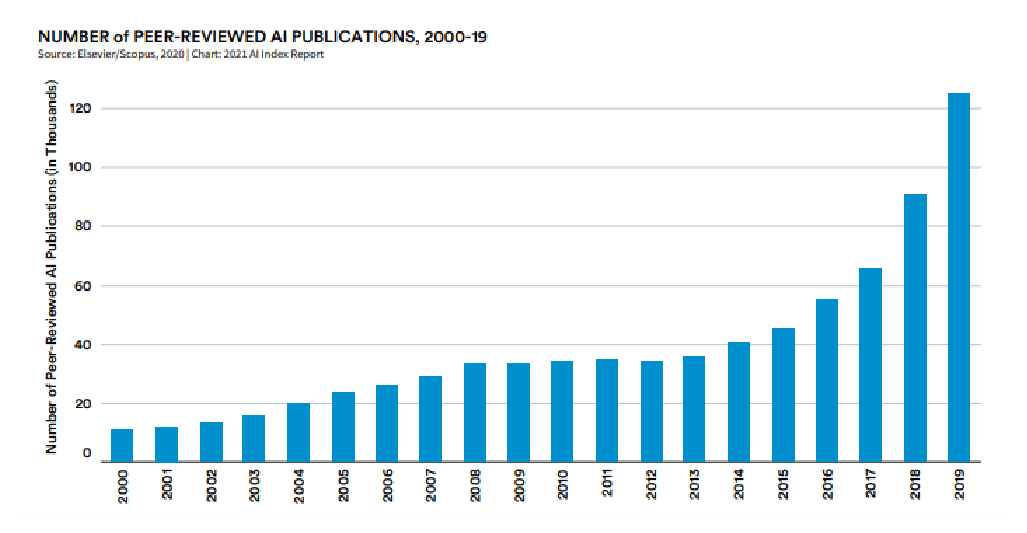
\includegraphics[scale=0.9]{images/chapter_1/AI_report.eps}}
\caption{Number of Peer-Reviewed AI Publications, 2000-2019 \citep{zhang2021ai}}
\label{fig:Number of Peer-Reviewed AI Publications}
\end{figure}


\subsubsection{Review of opportunities for the manufacturing industry}

In this section, we presents the result of a literature review we conducted to highlight some of the possibles applications where the Machine Learning could be applied in order to create value for the manufacturing companies. This study should not, in any case, be considered as an exhaustive list of possibilities. Results are summarised in table \ref{tab:ai_benefits}. 

\begin{table}
\label{tab:ai_benefits}
\begin{tabular}{|l|p{6cm}|p{4cm}|}
\hline
%
Domain &
  Benefits &
    Bibliography \\ \hline
% Quality Optimization
Quality Optimisation &
  Decrease the product failure rate at the end of the production line. Optimise key performance index of the final product to meet customer needs. &
    \citep{lieber2013quality, li2018ensemble, chen2008neural, nagorny2017quality, haeussler1996quality} \\ \hline

Maintenance &
  Increase the availability of the production line by preventing the breakdown of equipment in advance. Predict the risk of malfunction of the production line and arrange proactive maintenance. &
    \citep{nguyen2019new, lee2017application, einabadi2019dynamic, li2017intelligent, liu2016prediction}\\ \hline
Fault Diagnosis &
  Prognostic diagnose of production line failure event. Identify the malfunction part of the production line. Predict the abnormal behaviors of machines and equipment. & \citep{toma2020bearing, wong2006modified, chen2014fault, malik2017artificial, arabaci2010automatic} \\ \hline
Scheduling Optimisation &
  Logistic management of the production line, which can maximize the throughput of the production line. Buffer control and product routing management. & \citep{morariu2020machine, woschank2020review, lolli2019machine, zhang2019review, gomes2016developing} \\ \hline
\end{tabular}
\caption{ML opportunities in Manufacturing}
\end{table}


\section{Research framework: The Extrusion Blow Molding} \label{Research framework: The Extrusion Blow Molding}

The industrial process taken into account for our experimental setting is the Extrusion Blow-Moulding process. Extrusion blow molding is a process used to form hollow thermoplastic objects (especially bottles and containers). The process takes a thin-walled tube called a \textit{parison} that has been formed by extrusion, entraps it between two halves of a larger diameter mold, and then expands it by blowing air into the tube, forcing the parison out against the mold. The outside of the thin-walled part takes the shape of the inside of the mold \citep{poli2001design}.

\begin{figure}
\centerline{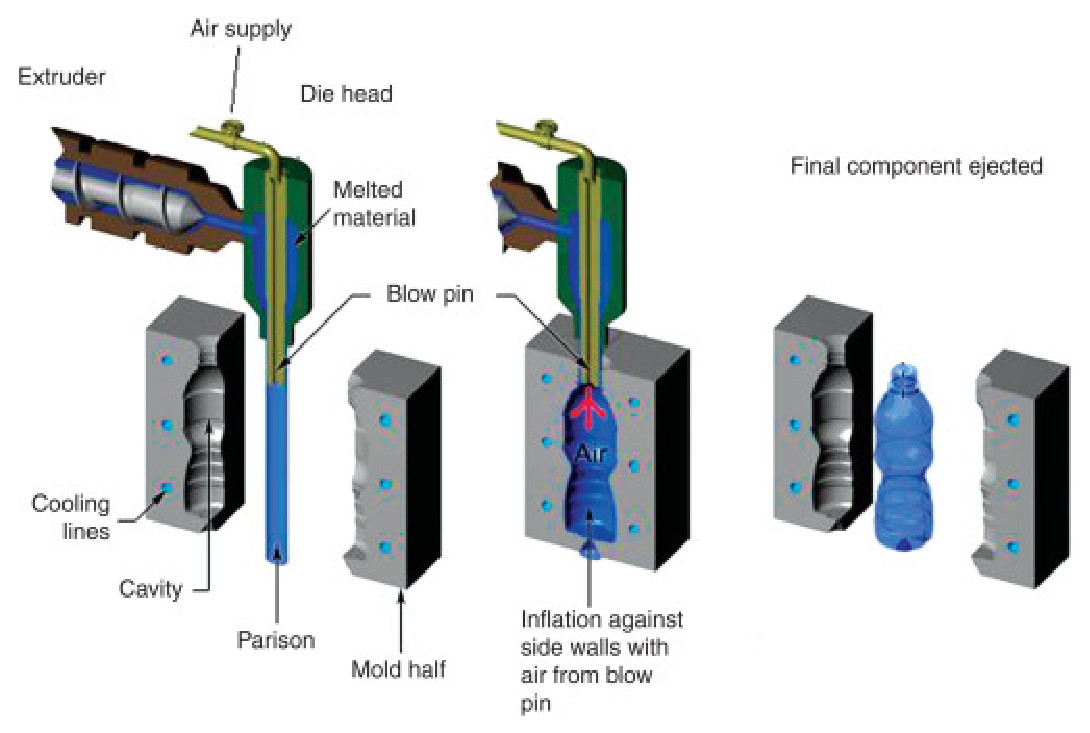
\includegraphics[scale=0.75]{images/chapter_1/extrusion_blow_molding.eps}}
\caption{Extrusion Blow-Molding \citep{goodship2015design}}
\label{fig:Extrusion Blow-Molding}
\end{figure}

As easily guessed by the name, the Extrusion Blow-Molding process is composed of two sub-processes: Extrusion and Blow-Molding.

\begin{itemize}
    \item \textit{The Extrusion:} The Extrusion is a continuous-flow process where a plastic material feedstock is fed through a hopper onto a feeding transfer screw. The thermal energy provided by the heating clamps as well as the mechanical energy provided by the screw rotation allows the melting of the plastic material.The die will typically create a tubular extruded cross-section, round or oval depending upon the final shape of the finished blow molded part. The melt is extruded through an annular die of adjustable gap, to form a hollow cylindrical membrane known as a parison. The die gap is the distance between the inner mandrel and the outer bushing. The gap can be varied during the extrusion, due to the tapered nature of the die, by moving either the mandrel or the bushing in a vertical direction. The process of variable die gap extrusion is referred to as parison programming and is utilised to manipulate the thickness distribution in the final part \citep{diraddo1993profile}.
    \item \textit{The Blow-Molding:} Unlike Extrusion, Blow-Molding is a discontinuous-flow process. In extrusion blow moulding, the parison is vertically suspended in the air during which time two mould halves enclose it by the action of a pneumatic or hydraulic mechanism. Internally applied air pressure causes the parison to inflate and take the shape of the inner parts of the molds. Once the blow operation is completed and the part has frozen suitably for ejection, the mold opens and the part is ejected, allowing the extruded parison to be extruded through the mold for the next cycle. 
\end{itemize}

Each phase has parameters that influence the subsequent phases and, ultimately, the characteristics of the finished product. The multiple phases mean that the number of parameters that can be adjusted on the process is fairly high. It is possible to fine-tune temperatures, screw speeds and throughputs for the Extrusion, as well as the  pressure curves, molds opening and closing times for the Blow-Molding phase. In addition, the Extrusion Blow-moulding process has a certain dynamic: it takes a certain amount of time for the adjustment of one of the process parameters to have an effect on the products. This dynamic is mainly due to the thermal inertia of the solid tooling.
One of the most critical part of the process is the parison formation. In fact, the dimensions of the blow molded article are directly related to the dimensions of the parison. Furthermore, the thermo-mechanical history of the material during the parison formation stage and the resulting weight and diameter distribution of the parison have a great influence on the characteristics of the subsequent inflation and cooling stages. The shape and the dimensions of the parison are the result of complex interactions between the molten ploymer and the thermo-mechanical conditions that influence the melt after it leaves the extruder die. Parison formation it is affected by two phenomena knows as \textit{swell} and \textit{sag}. Parison swell, occurring both in diameter and thickness, is due to the nonlinear viscoelastic deformation of the polymer melt in the extrusion die. Sag is caused by gravitational forces that act on the suspended parison \citep{huang2002prediction}. A high degree of swell could lead to molded articles which are to heavy and uneconomical, on the other hands, very low swelling could yield incomplete parts of low weight with unacceptable wall thickness.

There are many variations of this process including equipment made to extrude multiple parisons simultaneously, equipment that can extrude multiple layers within the same parison, equipment with rotary capability that will hold several molds and can provide a continuous nonstop process. Moreover, the extrusion blow-molding process can be split into two subcategories: intermittent extrusion blow molding and continuous extrusion blow molding. With intermittent extrusion blow molding, the extruder runs for a designated amount of time and fills a reservoir with plastic. Once the the reservoir has been filled, a plunger is activated and pushes the material from the reservoir through the extrusion head. On the other hand, in continuous blow-molding, the plastic is extruded permanently in a continuous manner while the machine runs.

In the context of this thesis project we have mainly worked with a continuous Extrusion Blow-Molding process, whose finished products are obtained from the overlay of multiple plastic layers. This particular type of Blow-Molding process takes the name of \textit{Co-extrusion}. Co-extrusion was born out of the need of reduce the permeability of fuel tanks. The steps for producing a multi-layers plastic product are the same as those used by the traditional single layer process, except for the number of extruders involved in the manufacturing process. Up to six extruders can be used simultaneously to melt different plastic materials. The goal is to create a multi-layer tank with the use of different material, as shown in
Figure \ref{fig:Co-extrusion Process}

\begin{figure}
\centerline{\includegraphics[scale=0.55]{images/chapter_1/coextrusion.png}}
\caption{Co-extrusion Process}
\label{fig:Co-extrusion Process}
\end{figure}

The Extrusion Blow-Molding constitutes one of the various stages necessary to produce the finished part. The stages needed to manufacture a finished part may vary depending on the type of product made. For instance, a fuel tank container, a plastic bottle or a plastic bumper may requires different post-production processes. Further information on how a fuel tank is produced are available in Appendix \ref{Full production process}. As far as our thesis work is concerned, we will only focus on The Extrusion Blow-Molding stage.

TALK ABOUT BATCH PRODUCTION


\subsection{The key parameters of the Extrusion Blow-Molding} \label{The key parameters of the Extrusion Blow-Molding}

The Extrusion Blow-Molding is a manufacturing process that requires the fine-tuning of multiples adjustable parameters in order to put the manufacturing process in the conditions to produce the final part. One of the most critical process parameter involving the Extrusion sub-process is the material throughput. Controlling the amount of material passing through each extruder is crucial for the following to reasons:  
%
\begin{itemize}
    \item It affects the cycle time. The throughput affects the ejection rate of the parison and therefore the cycle time. A cycle time reduction results in an higher manufacturing rate.
    \item The throughput ratios among the different 6 extruders should be controlled to ensure the correct amount of material on each of the 6 layers composing the tank thickness.
\end{itemize}
%
The throughput depends mainly on the rotation speed of the extruder and slightly on the extruder temperature. The temperature of the extruder affects the melting of the plastic material and the material fluidity may change. Depending on the material fluidity the throughput may change given the same extruder speed. For what has been said so far, controlling the temperature of the extruder along the screw length is mandatory to ensure constant and repeatable melting condition and therefore ensure a constant throughput. Another important parameter, which play a key role in the Extrusion Blow-Molding manufacturing process, is the opening of the die gap of the \textit{Head} of the machine. By controlling the the percentage of opening of the gap during the cycle time we are able to distribute more or less material along the parison length. This operation is important to ensure to put enough material in parison zones that are most stretched during the blowing phase. Of course, the parison length plays a key role in ensuring that the material distribution is well positioned relatively to the molds position. Unfortunately, in the production process in question, there is no control system for measuring the parison length. In continuous Extrusion Blow-Molding is the cycle time which triggers the blowing cycle.   

With regard of the Blow-Molding sub-process, the most critical parameters are the blowing pressure, or better the blowing pressures, since there exist 4 different air blowing circuits, the cooling water temperature and throughput. The blowing pressure ensure the parison to inflate and take the shape of the inner parts of the molds. Without enough air pressure the plastic material does not adhere to the molds surface preventing the correct material cooling. In the same way, the amount of water passing through the cooling circuit, as well as its temperature, affect cooling capacities of the molds. The following table resumes the list of the key parameters, identified together with process experts, of an extrusion blow-molding process.

\begin{landscape}
\begin{table}[]
\caption{Blow-Molding Key parameters}
\label{tab:key_parameters}
% \begin{adjustbox}{width=\textheight}
\begin{tabular}{|l|l|l|l|l|l|}
\hline
\textbf{Process}      &  \textbf{Parameter}                    & \textbf{Unity of measure}                  & \textbf{Value range}   & \textbf{Description}                                    & \textbf{Dependencies} \\ \hline
Extrusion    & Speed*                       & RPM                               & [0, 90]       & Rotation speed of the screw                               &              \\ \hline
Extrusion    & Throughput*                  & Kg/h                              & [0, 400]      & Material throughput in the extruder screw                 &  Speed, Temperatures            \\ \hline
Extrusion    & Melt Pressure*               & \% of the motor nominal torque    & [0, 450]      & Pressure at the end of the extruder screw                 &              \\ \hline
Extrusion    & Feeding Temperature*         & °C                                & [0, 100]      & Extruder temperature at the entrance of the extruder      &              \\ \hline
Extrusion    & Melt Temperature*            & °C                                & [0, 250]      & Extruder temperature at the end of the extruder          &              \\ \hline
Extrusion    & Cycle time                   & s                                 & [60, 120]     & Tank production cycle time                                &              \\ \hline
Extrusion    & Parison profile              & \% of the opening of the die gap  &               &                                                &              \\ \hline
Extrusion    & Parison length               & mm                                & [0, 3000]     & Length of the parison during the extrusion     &       \\ \hline
Blow-Molding & Blowing pressure**           & bar                               &               & Blowing pressure inside molds                                               &              \\ \hline
Blow-Molding & Cooling water temperature    & °C                                &               & Temperature of the cooling water (molds)                                               &               \\ \hline
Blow-Molding & Cooling water throughput     & Kg/h                              &               & Throughput of the cooling water (molds)                                               &              \\ \hline
\end{tabular}
% \end{adjustbox}
\end{table}
\footnotesize{$^*$ For each extruder, $**$ There exist 4 different blowing circuits}\\
\end{landscape}


\subsection{The key quality characteristics of a blow-molded fuel tank} \label{The key quality characteristics of a blow-molded fuel tank}

Quality Control is generally expressed as a management activity verifying the conformity of the process and the product/service to the requirements that constitute its quality standard. The ISO 9000 standard defines quality control as "A part of quality management focused on fulfilling quality requirements" \citep{iso9000}. In the industrial context taken into account the requirements are defined by the customers. Several characteristics are measured on the product and compared with the customer requirements, if the measures are compliant with the customer specifications the part can be sent to the customer, otherwise the part have to be rejected. In Blow-molded parts the material distribution all over the part surface plays a key role in ensuring that the finished product meets customer specifications. In the framework of the Extrusion Blow-Molding process, we are mostly interested in the dimensional/geometric characteristics. In fact, the main purpose of the quality control involving the blow-molded part is to asses the integrity of the plastic shell. The thickness of the tank over the whole surface must be enough to ensure the robustness of the part and therefore its safety, while avoiding an excessive and unnecessary weight of the finished product. Measuring the thickness of a blow-molded part over its entire surface is trivial because most of the blow-molded parts are hollow, which limits how the thickness can be measured. Moreover, the thickness is relatively small, with value ranging from $3$ to $8$ millimetres. This requires the use of measuring instrument with a precision of at least $0.1$ millimetres.

\paragraph{Background in thickness measurement}

Traditional methods to measure the thickness of hollow parts involve the use of ultrasonic measuring instruments that provide satisfactory results while avoiding the destruction of parts. The main idea of \textit{Ultrasonic Thickness Measurement} (UTM) is to measure the time needed for the ultrasonic wave to traverse the material. Some of the advantages of UTM over other nondestructive methods are:
\begin{itemize}
    \item the possibility to measure parts with just one accessible surface,
    \item no need for laboratory conditions,
    \item its high sensitivity and accuracy.
\end{itemize}
 
Although these methods are extremely high-performance for sample quality control, they present a major drawback: they cannot be used for online measurement. The measurement of a large number of points, which is necessary to estimate the distribution of the material over the entire surface, is time-consuming and cannot be applied online in production. Hence, the quality control of the thickness can only be carried using a sampling approach. Recently, new technologies involving the use of terahertz waves have been developed to accurately measure the thickness of materials without any contact with the material itself. These methods have proven to be extremely powerful for measuring the thickness of automobile paint \citep{su2014terahertz,krimi2016highly}, or pharmaceutical tablets \citep{may2011terahertz}. Of all the methods found in the literature, terahertz-based systems seem to be the only ones that can be used to perform real-time thickness measurement, but in order to use it in real-time, the measurement sensor must be installed on a robot, or collaborative robot, which can significantly affect the price of the complete measurement solution.

Another well-known technique for measuring thickness of parts is \textit{Computed Tomography} (CT). Typical areas of use for CT in industry are in the detection of flaws such as voids and cracks, and particle analysis in materials. In metrology, CT allows measurements of the external as well as the internal geometry of complex parts. As stated by \citet{de2014industrial}, CT is particularly suitable to investigate molded polymer parts, thanks to the good penetrability of X-rays in these materials. Even if CT-based techniques are extremely powerful, they require laboratory conditions and  do not lend themselves well to real-time thickness control. Moreover, this equipment may be very expensive, questioning its profitability.
%
Eddy current testing, widely applied for the non-destructive thickness measurement of metallic parts \citep{cheng2017thickness,mao2016thickness,wang2015noncontact,yin2007thickness}  is also non-destructive, but cannot be used as polymers composing the blow-molded part are not conductive.

In the last decades,\textit{Thermal Imaging}, a non-contact technology capable of measuring large surfaces in a single shot, has been studied as a possible method to infer the thickness of a solid element. \citep{sun2003method,sun2006analysis,choi2008quantitative,benitez2008definition,zeng2012absolute,li2018thickness,he2013eddy}. Among the most widely used thermal imaging approaches we can mention: \textit{Pulsed thermography} in which a brief controlled thermal stimulation pulse is applied on the tested piece, \textit{Step heating thermography} in which a continuous, uniform heat flow is applied for a long period, and \textit{Lockin thermography} in which a periodic heat input is used. The main idea behind all these approaches is to transfer energy to the test piece and to monitor its surface temperature evolution over time. In flash thermal imaging, for example, some flash lamps provide the thermal impulse, and the infrared camera monitors the surface-temperature decay on the heated surface. On the other hand, step-heating thermal imaging is using a long pulse of low intensity heat stimulation. Unlike pulsed thermal imaging, step-heating technology monitors the temperature raise over time while the heat energy is transferred to the test piece. The proposition of alternatives technologies, such as thermal imaging, to measure the thickness of the tank is one of the major contributions of this research work and the proposed approach will be presented in detail in chapter \ref{Thickness inference using thermal imaging}.

Due to the impossibility to measure the thickness of 100\% of the part produced, in practice, weight is often measured as an alternative. The weight is an indicator of how much material is composing the part and allows for an overall control of the quality of the part. The weight has a lower boundary to ensure that sufficient material is composing the tank and an upper boundary to avoid unnecessary weight of the finished product. Unlike the thickness, which has to be measured in several areas of the tank and cannot be carried out online for all the parts, the weight requires a simple weight scale, placed in the area where the blow-molded part is discharged. 

In order to produce a complete fuel system (compare appendix \ref{Plastic Omnium}), other manufacturing process are required after the Extrusion Blow-Molding (compare appendix \ref{Full production process}). Operations such as components welding or the assembly of pieces require further quality checks. The deepening of any quality control that does not directly concern the Extrusion Blow-Molding is out of the scope of this research work. The following table resumes the two quality characteristics of a blow-molded part we are interested in, and which must be monitored to ensure that the parts produced comply with the customer requirements. 


\begin{table}[]
\caption{Quality indicators of a blow-molded fuel tank }
\label{tab:quality_inidcators}
\begin{tabular}{|l|l|l|p{3cm}|}
\hline
\textbf{Quality characteristic} & \textbf{Unity of measure} & \textbf{Value range} & \textbf{Description}                                                 \\ \hline
Global Thickness           & mm                        & {[}3, 8{]}           & Thickness of the part measured in several critical areas of the tank \\ \hline
Weight & Kg & {[}6, 14{]} & Weight of the blow-molded tank \\ \hline
\end{tabular}
\end{table}




\section{Quality control and Process Monitoring in the Extrusion Blow Molding process: a state-of-the-art (THIS SECTION SHOULD BE IMPROVED --> INTEGRATE AMELIE FEEDBACK)} \label{state-of-the-art}

Since we are interested in improving the overall quality of the part produced through the Extrusion Blow-Molding process, a first work of literature review has been done to identify previous works in this domain. The literature review have been carried out using three different databases: \textit{Scopus}, \textit{Google Scholar} and \textit{Crossref}.

The global research query used to find potential interesting articles is the following:

\begin{verbatim}
    ("extrusion blow molding"  OR  "extrusion blow-molding"  OR
    "extrusion blow-moulding"  OR  "extrusion blow moulding" )  
    AND   ( "process control"  OR  "process monitoring"  OR
    "quality control"  OR  "quality prediction"  OR  "anomaly detection" )
\end{verbatim}

Subsequently, a screening exercise was carried out to select only the most interesting articles relevant to our scientific problem. Figure \ref{fig:wordcloud} highlights the recurring words in the title and abstract of the retained articles. 

\begin{figure}
\centerline{\includegraphics[scale=1]{images/chapter_2/wordcloud.png}}
\caption{Most recurrent words in article titles}
\label{fig:wordcloud}
\end{figure}

The bibliographical research work has highlighted two main strategies to improve the quality of the blow-molded parts:

\begin{itemize}
    \item Expertise-based approaches: The first approach makes use of physics and simulation to model the manufacturing process and to fine tune process parameters given the simulated final part characteristics. 
    \item Data-driven approaches: As the production process is complicated to be modelled physically, most of the work carried out previously makes use of data-driven methods to understand what process parameters affect the most the quality of the blow-molded parts. The patterns discovered within data allow a subsequent optimisation of the process parameters.
\end{itemize}


In the remaining part of the current section, we will investigate the approaches proposed in the literature and we will discuss the possibility of using this methods in our industrial context. The following two subsections will provide more details about the two identified research strategies: expertise-based approaches (\ref{Expertise-based approaches}) and data-driven approaches (\ref{Data-driven approaches}). 

\subsection{Expertise-based approaches} \label{Expertise-based approaches}

Different strategies have been used to model the whole process that is the parison extrusion, clamping, inflation and cooling. \citep{lee1996prediction} used a finite element model of thin film to simulate blow molding processes, and applied the feasible direction method to minimise the parison volume at the constraints of part thickness. The proposed parison design simulation is composed of the following stages. The finite element model predicts the wall thickness of the blow-molded part from a given preform thickness. The resulting wall thickness distribution of the part is submitted to the optimisation model to generate a new preform thickness profile. The new preform design is compared with the old one. If there is any improvement, the new preform design is again passed to the finite element model, and the loop is repeated until no further design improvement can be achieved. Author showed that the presented approach makes the optimisation algorithm more efficient and reduces the computational requirement drastically. 

Others expertise-based methods rely on iterative fine-tuning loop involving the prediction of the final part characteristics, such as the weight or the thickness. Two approaches, with regard to material behaviour during inflation, have been applied for the prediction. The first method assumes that the polymer melt behaves as a viscous or a viscoelastic fluid, whereas the second method assumes that the melt behaves as an elastic solid. The assumption that the parison behaves as a viscous or a viscoelastic fluid results in a very complex computational formulation. \citep{poslinski1990nonisothermal} treat the parison as a Newtonian fluid subject to a non-isothermal inflation. Parison position and cooling during the inflation are predicted as a function of time. Some experimental final part thickness distributions are obtained and compared to simulation results for a simple mould geometry and a constant initial thickness preform. Also, the inherent elastic nature of the polymer melt is not considered, since the formulation assumes a Newtonian fluid. \cite{ryan1982dynamics} as well as \citep{khayat1992inflation} assume a viseoelastic behaviour of the polymer melt. The inflation is modelled as a dynamic process, predicting the parison inflation as a function of time. A free inflation was considered. Attempts with confined inflation, that is employing a mould geometry, have not been handled to date. 
The approaches discussed in \citep{poslinski1990nonisothermal}, \cite{ryan1982dynamics} \citep{khayat1992inflation} are interesting but make very strong assumptions or deal with very particular cases.

In 2008 \citep{attar2008manufacturing} proposed an approach to assist the development phase of a new product and to optimise the weight of the part and its thickness distribution. Firstly, simulation of the extrusion blow moulding process and preliminary experimental trials were performed concurrently to assist in the development of the part. Once the numerical modelling of the part was done, improvement of the production process was performed based upon the desired objective function, i.e., a uniform part thickness distribution and/or minimal part weight. The optimisation was performed in two sequential steps, weight optimisation then thickness optimisation, by the systematic manipulation of the operating conditions, such as the parison dimensions. A process modelling methodology was employed to demonstrate the reduction in the part development time using the new model-based approach (Figure \ref{fig:workflow_development_process_optimisation}).
\begin{figure}
\centerline{\includegraphics[scale=0.6]{images/chapter_2/optimisation_flow.png}}
\caption{Workflow for development process optimisation \citep{attar2008manufacturing}}
\label{fig:workflow_development_process_optimisation}
\end{figure}
It is a trial and error process, which is time-consuming and produces a lot of material scrap. On the other hand, the concurrent process optimises parameters virtually, and therefore, eliminates scrap, machine downtime and the need for experimental optimisation. The results demonstrate that there is a significant reduction in span time and in effort, since much of the delay and rework is eliminated using the simulation-based development process.


\subsection{Data-driven approaches} \label{Data-driven approaches}

\citep{diraddo1993line} have employed an entirely different methodology as a forward predictor of the inflation process. Neural networks are used for the on-line prediction of the final part thickness distribution from the initial process conditions. The Fully connected neural network inputs include the initial parison thickness and temperature profiles, the bottle mold geometry and a rheological parameter representative of the raw material. The neural network is trained by employing a gradient descent optimisation regression approach and mapping a broad range of output and input data. Once trained, the algorithm is capable of predicting outputs based on new inputs. Authors claimed that the proposed data-driven methods has several advantages over simulations based methods. On first principles include faster response and the network’s ability to update a model to account for process shifts. Neural networks do not allow for an understanding of process fundamentals, they require a great deal of experimental data for the training procedure and problems can arise with extrapolation beyond the range defined by the experimental data. Therefore, the methodology is better suited for on-line applications, where fast response and following of process shifts is crucial. The same authors proposed in \citep{diraddo1993modeling} another have employed neural networks for the modelling of the process with the inverse formulation. Compared to the previous approach they tried to predict the initial parison thickness given the thickness of the final part. It would be valuable to determine the process conditions given the specified final part thickness distribution. The proposed approach was, in most cases, able to predict the constant thickness parison profile required for the specified part thickness distribution.   

Another interesting approach have been carried out by \citep{ramana2013data}. They propose to use data mining techniques to identify the factors that significantly affect quality, modeling relationships between input attributes and target attribute (yield, quality, performance index etc) and predicting quality levels of given input attributes. Clustering analysis have been initially applied on process data to split the entire population in different clusters. The cluster analysis made it possible to categorise the data into different families. By comparing the results of the cluster families analysis with the data labels, they prove that reject part are categorised in different clusters than parts conforming to customer specifications. Naive Bayes and Decision Tree has been then applied with the main purpose of classify the quality of the part given the input parameters. The process parameters used as input data are: the process cycle time, the extruder temperatures in different zones, the Extrusion Die temperature, the expulsion time, the parison length, the parison shape the blowing pressures as well as the inflation time. Naïve Bayes and clustering models were found to have better accuracy than Decision Trees in the evaluation performed by standard lift chart while predicting process parameter values that result in acceptable products. The knowledge driven and proactive decisions have been implemented in quickly setting process parameters and their range of values that resulted in increased output of high quality products and significantly reduced the scrap.

\subsection{Discussion} \label{Discussion}

The scientific literature pointed out previous works in the domain of Extrusion-Blow Molding process and quality optimisation. Two different approaches have been presented: expertise-based and data-driven approaches. Both have advantages and disadvantages. Expertise-based approaches need strong assumptions or simplification to account for the overall process complexity. Data-driven methods are faster and they can be used online. On the other hand, they require a great deal of experimental data for the training procedure and problems can arise with extrapolation beyond the range defined by the experimental data. Both methods try to predict the quality of the final part given the process conditions with the main purpose of fine-tuning the manufacturing process. 

This bibliographical research work has made it possible to highlight two other fundamental aspects:

\begin{itemize}
    \item Due to the complexity of the studied production process, most recent approaches to improve the quality of the manufactured parts or to improve the process control make use of data-driven methods.
    \item None of the articles considered deals with the process of multi-layers Extrusion Blow-Molding (Co-extrusion). Extrusion-Blow molding scientific literature mainly focus on plastic bottle or simple plastic containers which are commonly produced through mono-layer extrusion blow-molding process. For this reason, some of the proposed methods are not directly applicable to our production process. For instance, the approach presented by \citep{diraddo1993line} for evaluating the geometrical dimensions of a plastic bottle is really interesting. On the other hand, among the input process data used as predictors, they use the material throughput exiting the extrusion head as well as the rheological parameter representative of the raw material. This information is missing from the production process under consideration and any modification to the machine to retrieve the missing information would not be possible for technical and economical reasons.
    \item Previous research work deals mainly with the development phases of the products. Only a few of the literature works are concerned with improving the quality of the part in production. When the machine is properly set, the scrap rate is close to $0$. On the other hand, there are certain internal or external factors which can cause the production of non-conforming parts. It would be interesting to identify in real-time, or even prevent, these factors that can lead to a degradation of the product quality. This would allow a faster process adjustment and even greater reduction of the scrap rate.
\end{itemize}

Starting with the results obtained by \citep{diraddo1993line} and \citep{ramana2013data}, and with the advancement of machine Learning techniques in the last decade, we decided to move our attention towards data-driven methods. Supported by the scientific literature, and taking into account technological advances in the domain of the data acquisition in the manufacturing environment, we claim that data-driven methods are the right tools to investigate the interactions between Extrusion Blow-Molding process data and the corresponding product quality data. We claim that this is particularly true in a Co-extrusion production process, where there are six extrusion screws, extruding 6 different types of polymers with different physical-chemical properties. Physically modelling the production process would be quite complicated as too many assumptions would have to be taken into account. The interest of using data-driven methods is also confirmed by the scientific literature of the last years involving quality improvement. Data-driven methods for product quality control have been successfully applied in multiple domains, from steel industry \citep{lieber2013quality,li2018ensemble} to plastic industry \citep{chen2008neural,nagorny2017quality,haeussler1996quality,tellaeche2013machine,sharma2017taguchi} and to the semiconductor manufacturing processes \citep{melhem2016regression,lenz2013data,jiang2020novel}.

\section{Research objectives and methodology}

Because manufacturing processes are becoming more and more complex, and the high level of requirement in the automotive industry regarding safety and environmental impacts, Plastic Omnium is continuously seeking for innovation throughout its different projects that allows the company to remain leader in its field. For Plastic Omnium, the Industry 4.0 paradigm can provide a new way of looking at performance, with a more precise and immediate vision (based on real-time indicators) of the entire production chain, but also the optimisation of production through the use of data-driven methods. An in-depth presentation of the activities of Plastic Omnium is available in Appendix \ref{Plastic Omnium}. For Plastic Omnium the are four main pillars driving the Industry 4.0 revolution:

\begin{itemize}
    \item \textit{Smart Factory}: it refers to the set of initiatives that enable for a real-time traceability of what is happening inside production plants. With a real-time system, raw materials, work in progress and finished products are bar coded and tracked throughout the manufacturing process. The digitisation of the data allows also for a better monitoring of the production performance.
    \item \textit{Digital industrialisation}: it refers to the set of initiatives that make use of Virtual Reality (VR) and Digital twin models to reduce the deployments costs of new machine and to optimise the plant machine layout. Others initiatives aims to optimise the ergonomics. 
    \item \textit{Predictive quality}: it refers to the use of data-driven methods to decrease the product failure rate at the end of the production line. This topic covers also all the initiatives that aims for improving the quality control and reduce the destructive tests on the parts for quality control reasons.  
    \item \textit{Predictive maintenance}: it refers to the use of data-driven methods that are meant to analyse equipment status and forecast when maintenance should be performed. Predictive maintenance aims to reduce the number and the duration of the unplanned down-times and to optimise the maintenance operations.
\end{itemize}
%
Figure \ref{fig:pillars} shows how these topics integrate within the research environment of Plastic Omnium.
%
\begin{figure}
\centerline{\includegraphics[scale=0.50]{images/chapter_1/Digitalisation_pillars.png}}
\caption{Industry 4.0 pillars for Plastic Omnium}
\label{fig:pillars}
\end{figure}
%
Among the different topics, this research work will focus on the "Predictive Quality" topic. For an equipment manufacturer like Plastic Omnium Clean Energy Systems (CES), bad or ``scrap'' parts are very expensive for the company. The “Cost of Non-Quality” (CNQ) is one of the key indicators most used to evaluate the production capacity of a company. Therefore, this research work aims at looking for the best way to use the collected process data on the machines and the corresponding product quality data in order to propose a data driven approach able to infer the quality of a product. The choice to use a data-driven approach is motivated by an ever-increasing availability of data within the manufacturing plants as well as from what has been said in the previous section (compare section \ref{state-of-the-art}). Using the data that is already available within the company will be an important part of the global study, because it will be the first input going into the developed monitoring system. In the case of Plastic Omnium CES, the data coming from the systems \textit{PES} (Production Execution System) and \textit{DASIP} (Data Acquisition for the Supervision of Industrial Process) will be important. The two systems allow for the traceability of the produced parts as well as a monitoring of the different events happening on the plant’s machines (for PES), and DASIP is monitoring key parameters of the production processes. Other data sources will be investigated during this work.

This system will help detecting product non-conformities to plan the corrective actions accordingly. The expected benefits are:

\begin{itemize}
    \item The reduction of product non-conformities. 
    \item The overall quality control improvement.
    \item Process improvement. In fact, the product quality improvement cannot be obtained without working on the manufacturing process. This will help for a better comprehension of the Extrusion Blow-Molding Process. 
\end{itemize}

To reach the final objective of reducing the scraps and the non-quality costs, a data-driven methodology will be proposed in order to implement an inference system. The methodology is articulated around three principles consecutive stages, to answer as best as possible the research objective:

\begin{enumerate}
    \item Proposal of a general framework to deal with ``Predictive Quality'' topics 
    \item Application of the proposed methodology to the industrial context studied
    \item Proposal of a decision-making system 
\end{enumerate}

Each of the four stages requires to overcome either some scientific or industrial issues or obstacles. In the scope of this thesis, we will only be able to work on the first three topics, although some elements concerning the last stage will be discussed in chapter \ref{Contributions and perspectives}. In the following paragraphs, we will review for each stage those that for us are the main scientific and industrial obstacles to overcome.

\paragraph{Proposal of a general framework to deal with ``Predictive Quality'' topics}

During the first stage, we will leverage scientific literature to propose a general methodology to deal with all Predictive Quality topics. On an industrial point of view, this first stage requires the identification of all the necessary tools and methods needed to conduct a project from start to finish.

\paragraph{Application of the proposed framework to the industrial context studied}

The second stage will require the application of the proposed framework to the industrial use case taken into account. Once the critical data needed to answer our research question are identified, a Machine Learning algorithm will be applied to try to infer the quality of a part given the set of input parameters identified in the previous stage. From a scientific point of view, this stage will require to identify or build an efficient and robust Machine Learning algorithm able to model the transfer function which relates the input process data and the output quality data. 

\paragraph{Proposal of a decision making system}

The last stage will involve the implementation of a decision-making system able to asses the quality of a produced part and, if necessary, to reject it. The system should be able to communicate with the systems already in place, such as the \textit{PES} system, to declare the part as non-compliant and to alert quality and production teams to trigger corrective activities. 

% Figure \ref{} ADD REF resumes the three stages of our methodology as well as the most important scientific and industrial issues which have to be overcome.

\section{Conclusion}

In this fist chapter, we have described the context of our research project. Industry 4.0, holds the promise of increased flexibility in manufacturing, along with mass customisation, better quality, and improved productivity. The development of new technologies such as Machine Learning (and Deep Learning), IoT and Cloud Computing are opening up new perspectives in the manufacturing industry. The french automotive company Plastic Omnium, leader in the production of automotive plastic components aims to take advantage of the fast growing amount of data available in the manufacturing plants to improve the quality of the fuel tank produced through the Extrusion Blow-molding manufacturing process. The Extrusion Blow-Molding is a complex manufacturing process which is composed of two sub-processes: the \textit{Extrusion} and the \textit{Blow-Molding}. The Extrusion is a continuous-flow process where a plastic material feedstock is fed through a hopper onto a feeding transfer screw. The thermal energy provided by the heating clamps as well as the mechanical energy provided by the screw rotation allow the melting of the plastic material. The die will typically create a tubular extruded cross-section, round or oval depending upon the final shape of the finished blow molded part. Unlike Extrusion, Blow-Molding is a discontinuous-flow process. In extrusion blow moulding, the parison is vertically suspended in the air during which time two mould halves enclose it by the action of a pneumatic or hydraulic mechanism. Internally applied air pressure causes the parison to inflate and take the shape of the inner parts of the molds. The fuel tank produced through this manufacturing process must respect some dimensional and geometrical constraints to comply with the specifications. The thickness of the tank over the whole surface must be enough to ensure the robustness of the part and therefore its safety, while avoiding an excessive and unnecessary weight of the finished product. The scientific literature, involving the quality control and the process monitoring in the Extrusion Blow-Molding process, identifies two different ways of working on the topic of improving the quality of a blow-molded parts. The first approach mainly relies on expertise-based and expert system to optimise the manufacturing process. The second method makes use of data and data-driven methods to try to explain the variability of the quality of the final part given the input manufacturing process parameters. The limitations of the approaches proposed in the literature, as well as the motivations that have oriented us towards the use of data-driven methods have been discussed. Finally, the main research objectives as well as the research axes that will drive our research work are presented. In the next chapter, the methodology to deal Predictive Quality data, corresponding to the first stage of our methodology, will be presented.
